\documentclass[a4paper]{llncs}
\usepackage[utf8]{inputenc}
\usepackage[swedish]{babel}
\usepackage[hyphens]{url}
\usepackage{hyperref}
\usepackage[swedish]{cleveref}
\usepackage{marginnote}
\usepackage{framed}
\usepackage{booktabs}
\usepackage{xcolor}
\usepackage{pdfpages}

\usepackage[natbib,style=numeric-comp,sorting=none,maxbibnames=99]{biblatex}
\addbibresource{risksem.bib}

\usepackage{verbatim}
\let\solution\comment%

\pagestyle{plain}

% XXX translate to english, add enisa literature

\begin{document}
\title{Seminarium: Verksamhetsanalys och riskanalys}
\author{%
  Carina Bengtsson
  \and
  Lennart Franked
}
\institute{%
  Department of Information and Communication Systems\\
  Mid Sweden University, Sundsvall
}
\date{\today}

\maketitle

\section{Introduktion}
\label{sec:introduction}

Detta seminarium fokuserar på att diskutera vikten av en verksamhetsanpassad 
klassificeringsmodell, samt att praktiskt genomföra en enklare verksamhets- och 
riskanalys.
Utgångspunkten för seminariet är en klassificeringsmodell som ni kommer att 
utveckla inför seminariet.


\section{Syfte}
\label{sec:aim}

Syftet med uppgiften är:
\begin{itemize}
  % $Id$
\item develop an understanding of and gain practical experiences to design a
classification model.
\item  implement an organisational analysis as well as a risk analysis.

\end{itemize}


\section{Läsanvisningar}

% $Id$
% Author:	Daniel Bosk <daniel.bosk@miun.se>
Du ska inför skrivningen av detta PM ha läst dokumenten
\begin{itemize}
  \item \emph{Introduktion till metodstödet}~\cite{MSB2011itm},
  \item \emph{Säkra ledningens engagemang}~\cite{MSB2011sle}, och
  \item \emph{Projektplanering}~\cite{MSB2011p}.
\end{itemize}



\section{Utveckling av klassificeringsmodell}
\label{sec:work}

Genomförandet av uppgiften består av tre deluppgifter.
Den första delen handlar om att utforma en egen klassificeringsmodell, den 
andra om att använda den och till slut ska den förklaras.

\subsection{Utforma en klassificeringsmodell}
\label{sec:develop}

Utveckla en enklare klassificeringsmodell \emph{som är anpassad} efter den 
verksamhet du har blivit tilldelad:
\begin{itemize}
  \item universitet (myndighet),
  \item kommun, eller
  \item reseföretag (privat företag).
\end{itemize}
\begin{framed}\noindent
  Tips:
  \begin{itemize}
    \item Tänk på att olika verksamheter har olika krav och förväntningar på 
      sig.
      Utgå från de krav och förväntningar du har på organisationens 
      verksamhet\footnote{%
        Den triviala kravställningen \enquote{jag har inga krav eller 
          förväntningar} kommer naturligtvis inte att godkännas.
      } och diskutera gärna dessa i forumet i lärplattformen.
      Det finns även en överblick över några lagar som gäller en myndighet 
      i \citet[bilaga B]{MSB2011v}.
      Några av dessa gäller även för andra verksamheter.
    \item Titta på föreläsningsbilder, utgå från MSB:s modell eller använd 
      Google för att hitta exempel på hur andra har gjort för att få 
      inspiration till din klassificeringsmodell.
  \end{itemize}
\end{framed}

\subsection{Använda klassificeringsmodell}
\label{sec:use}
\noindent
Placera in följande fem informationstillgångar i din nyutvecklade 
klassificeringsmodell utifrån de krav du kommit fram till finns för din 
verksamhet:
\begin{enumerate}
  \item lönelistor,
  \item beslutsunderlag gällande verksamheten skickat via SMS,
  \item arbetsmaterial inför nästa års budget,
  \item loggar för inpasseringssystemet, och
  \item \enquote{kundregister}; kursdeltagare för universitetet, klasslista på 
    kommunal skola, resenärer till senaste Mexicoresan för reseföretaget.
\end{enumerate}
\begin{framed}\noindent
  Tips: Vid redovisning av denna uppgift rekommenderas det att skriva enligt 
  följande:
  \begin{center}
    \begin{tabular}{ll}
      \toprule
      \textbf{Område} & \textbf{Klass} \\
      \midrule
      Lönelistor  & K\(x\) \\
                  & T\(y\) \\
                  & R\(z\) \\
      \midrule
      Beslutsunderlag & K\(x^\prime\) \\
                      & T\(y^\prime\) \\
                      & R\(z^\prime\) \\
      \midrule
      \dots \\
      \bottomrule
    \end{tabular}
  \end{center}
  Där \(x\), \(y\) och \(z\) är de valda klasserna för konfidentialitet, 
  tillgänglighet respektive riktighet.
\end{framed}

\subsection{Förklaring av klassificeringsmodell}
\label{sec:explanation}
\noindent
Förklara hur du resonerade när du utformade din klassificeringsmodell, till 
exempel vad som gjorde att du valde de olika klasserna.
Ta gärna med vilka eventuella svårigheter du stötte på, vilka saker som var 
självklara, och vilka utvecklingsmöjligheter du ser med din modell.
Omfattningen bör vara maximalt 500 ord.


\section{Förberedelse för seminariet}

Genomförandet av seminariet består av tre delar motsvarande delarna 
i utvecklingen av klassificeringsmodellen.

Senast dagen innan seminariet ska du ha lämnat in en presentation i
form utav 1--5 bilder innehållandes din klassificeringsmodell, hur du valt
att klassicera dina informationstillgångar, samt vilka interna och legala krav
du utgått ifrån för respektive informationstillgång. Räkna med att du får max 5
minuter att presentera ditt arbete.

\subsection{Redovisning av klassificeringsmodell}
\label{sec:present}

En till tre personer i respektive grupp kommer att få förmånen att presentera 
sitt arbete.

\subsection{Användning av klassificeringsmodell}
\label{sec:use}

Några nya informationstillgångar kommer att ges under seminariet.
Ni kommer att delas upp i mindre grupper, där ni inom grupperna diskuterar er 
fram till vart ni vill placera dessa informationstillgångar i en utvald 
klassificeringsmodell.
Utvalda grupper presenterar därefter sitt förslag med tillhörande motivering.

\subsection{Riskanalys}
\label{sec:risk}

I samma grupper som ni jobbade med under \cref{sec:use}, ska ni nu utföra en 
riskanalys på en informationstillgång som seminarieledaren ger er.
Varje grupp ska komma fram till minst fem (5) hot mot vald 
informationstillgång som ska placeras i en riskmatris, samt ska ni för upptäckt
hot komma fram till ett åtgärdsförslag. Varje grupp ska sedan inför helklass presentera
de två hot som de anser vara mest kritiska. Detta ska övervägas genom att vikta sannolikheten
att hotet förekommer gentemot uppskattad frekvens.

\section{Examination}
\label{sec:examination}

Denna uppgift kommer att examineras genom ett skriftligt PM som lämnas in som 
ett PDF-dokument och genom aktivt deltagande under seminariet.
PM:et ska innehålla uppgifterna från \cref{sec:work}:
\begin{enumerate}
  \item utformning av klassificeringsmodell,
    \begin{solution}
      Betyg: F eller P.

      För att få godkänt krävs att man har en klassificering för perspektiven 
      \emph{tillgänglighet}, \emph{riktighet} och \emph{konfidentialitet}.
      Och att man på något sätt har minst en klass i varje perspektiv.
    \end{solution}

  \item användning av klassificeringsmodell, och
    \begin{solution}
      Betyg: F eller P.

      För att få godkänt krävs att man använt sin utformade 
      klassificeringsmodell, d.v.s.\ att alla givna informationstillgångar är 
      klassificerade utifrån tillgänglighet, riktighet och konfidentialitet --
      däremot kan vi nog aldrig säga att någon utförd klassificering är rätt 
      eller fel.
    \end{solution}

  \item förklaring av klassificeringsmodell, 500 ord.
    \begin{solution}
      Betyg: F-C.

      Principen för klassificering finns 
      i \emph{Verksamhetsanalys}~\cite{MSB2011v}, avsnitt 2.3 
      \emph{Klassificering av informationstillgångar}.
      Följande bör uppfyllas:
      \begin{itemize}
        \item Man bör få med att man tagit hänsyn till de förväntningar och krav 
          som finns på verksamheten (interna och externa krav), antingen legala 
          krav (mycket bra betyg) eller deras egna förväntningar (bra betyg).
          Eller både och (superbra betyg).
        \item Man bör på något sätt ha visat hänsyn till olika konsekvensnivåer 
          för verksamheten i de olika klasser som utformas.
          D.v.s.\ att de klasser som är utformade kan överföras till mer eller 
          mindre allvarliga konsekvenser för verksamheten vid brist på någon av 
          tillgänglighet, riktighet eller konfidentialitet.
        \item Ett bra komplement för föregående punkter är att ge förslag på 
          något som kan vara skyddsvärt för verksamheten, eller resonera kring de 
          \enquote{givna informationstillgångarna} tidigare i PM:et.
        \item Man bör vara reflekterande över utvecklingsmöjligheter och 
          svårigheter i uppgiften (visa att man förstår komplexiteten av 
          uppgiften).
      \end{itemize}
      Uppfyller de sista två punkterna bör de vara godkända.
      Uppfyller de dessutom de första två punkterna höjer det deras betyg 
      ytterligare.
    \end{solution}
\end{enumerate}

Dokumentet ska vara skrivet med akademisk svenska eller engelska och ha 
korrekta referenser.

Aktivt deltagande i seminariet krävs för godkänt betyg.
Detta innebär även att du inför seminariet måste lämna in de 1--5 bilder som 
nämndes ovan --- detta för ingen ska komma oförberedd.


\printbibliography{}


\appendix
%\section{Kompletteringsuppgift}
%
%Denna kompletteringsuppgift gäller för de som ej medverkat vid seminariet om
%verksamhets- och riskanalys.
%Utgångspunkten för uppgiften är den promemoria som behandlade området
%verksamhets- och riskanalys.
%
%\subsection{Genomförande}
%
%Genomförandet av kompletteringsuppgiften består av tre delar: tillämpning av 
%klassificeringsmodell för att klassificera informationstillgångar, jämföra 
%klassificeringar för olika verksamheter och till sist genomföra en riskanalys.
%
%\subsection{Använda klassificeringsmodell}
%\label{sec:use}
%
%Placera in följande två informationstillgångar i klassificeringsmodellen som du 
%själv utvecklat i promemorian, placera in dem utifrån de krav du kommit fram 
%till finns för din verksamhet:
%\begin{itemize}
%  \item hyreskontrakt och
%  \item verksamhetsberättelse.
%\end{itemize}
%
%\subsection{Jämföra klassificeringar}
%\label{sec:compare}
%
%Redogör för hur du skulle resonerat om du istället skulle ha klassificerat de 
%två ovan informationstillgångarna i de verksamheterna som du ej blev tilldelad 
%för PM:et för verksamhets- och riskanalys.
%Exempelvis om du blev tilldelad den kommunala verksamheten, då resonerar du 
%kring hur du istället skulle klassificera ovan givna informationstillgångar för 
%ett universitet och ett reseföretag:
%\begin{itemize}
%  \item Vad finns det för likheter och skillnader i klassificeringen för 
%    respektive informationstillgång?
%  \item Skulle respektive informationstillgång klassificeras som mer, mindre 
%    eller lika kritiska som för din ursprungliga verksamhet?
%\end{itemize}
%
%\subsection{Riskanalys}
%\label{sec:risk}
%
%Välj ut en av de två informationstillgångarna från uppgift~\ref{sec:use} för 
%att genomföra en riskanalys.
%Ange för vilken aspekt du gör analysen: konfidentialitet, tillgänglig\-het 
%eller riktighet.
%Identifiera minst tre hot och placera in dem i riskmatrisen.
%
%\begin{framed}\noindent
%  Tips:
%  \begin{itemize}
%    \item En riskanalys genomförs oftast på de informationstillgångar som anses 
%      vara med kritiska för verksamheten.
%      Exempelvis om du har verksamheten reseföretag, har fyra klasser i din 
%      modell och har klassificerat enligt följande:
%      \begin{center}
%        \begin{tabular}{ll}
%          \toprule
%          \textbf{Område} & \textbf{Klass} \\
%          \midrule
%          Hyreskontrakt & K2 \\
%                        & T2 \\
%                        & R3 \\
%          \midrule
%          Verksamhetsberättelse & K2 \\
%                                & T2 \\
%                                & \color{red}{R4} \\
%          \bottomrule
%        \end{tabular}
%      \end{center}
%      Då rekommenderas att göra en riskanalys \emph{gällande riktighet} för 
%      verksamhetsberättelsen.
%      (Ta då inte upp hot mot tillgänglighet och konfidentialitet.)
%
%    \item Använd gärna mallen i \cref{app:riskanalys} eller den i MSB:s 
%      dokument om riskanalys~\cite[bilaga A]{MSB2011r} för att redovisa ditt 
%      resultat av riskanalysen.
%    \item Exempelvis ett hot mot riktigheten i verksamhetsberättelsen kan vara 
%      att \enquote{någon utomstående ändrar medvetet i verksamhetsberättelsen
%      för att förvanska förra årets resultat, ändringen sker genom att
%      fysiskt sätta sig vid en dator som är olåst och göra ändringarna}.
%      \begin{itemize}
%        \item Uppskatta därefter konsekvensen av och sannolikheten för att 
%          detta inträffar i riskmatrisen.
%        \item Slutligen, beskriv vilka risker du tycker att verksamheten bör 
%          arbeta vidare med, och vilka risker du anser att man kan acceptera 
%          för tillfället.
%          (Använder du riskanalysmallen i \cref{app:riskanalys} räcker det 
%          med att du kryssar för det alternativ du vill använda dig av på 
%          respektive hot.)
%      \end{itemize}
%  \end{itemize}
%\end{framed}
%
%\subsection{Examination}
%\label{sec:Examination}
%
%Denna uppgift kommer att examineras genom \emph{ett} skriftligt dokument som 
%lämnas in i PDF-format.
%Om du väljer att använda mallar från MSB eller den i \cref{app:riskanalys} 
%måste du infoga dem i det dokument du lämnar in.
%Dokumentet ska innehålla uppgifterna från \cref{sec:work}:
%\begin{enumerate}
%  \item Använda klassificeringsmodell,
%  \item Jämföra klassificeringar, och
%  \item Riskanalys.
%\end{enumerate}
%
%
\section{Mall för riskanalys}
\label{app:riskanalys}

Dokumentet som följer finns även tillgängligt i lärplattformen i redigerbar 
form.

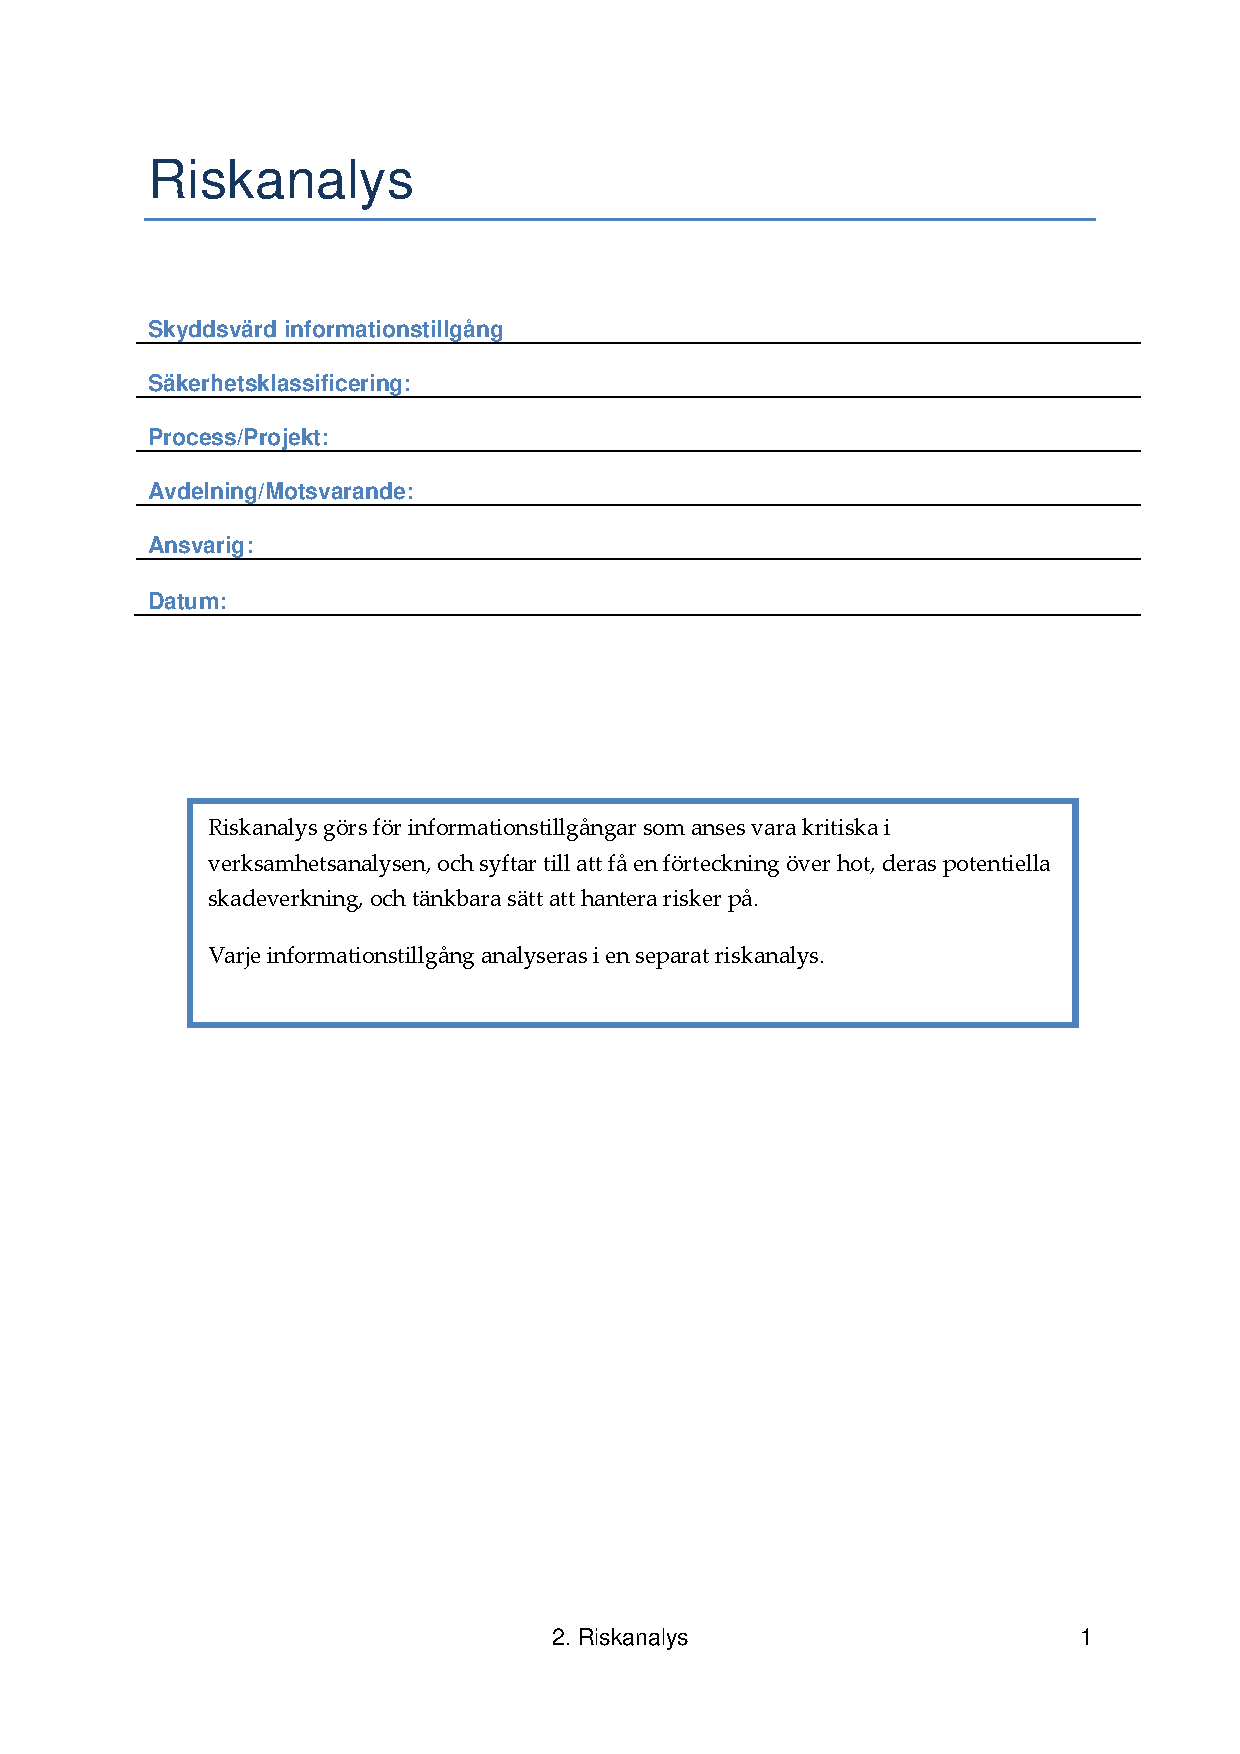
\includepdf[pages=-]{riskanalys-mall.pdf}

\end{document}
